\chapter{查看体数据}\label{ch:volume}
\index{Tishuju@体数据}

\chapterlead{原子结构告诉我们原子位于何处，体数据则描述空间中的数值如何变化。电荷密度、磁化密度以及其他标量场，都可以用等值面、切面或直接体渲染观察。本章以 CHGCAR、Cube 和 XSF 为例，介绍如何选择通道、读懂单位、比较图形，并导出适合报告与进一步分析的结果。}

\section{读懂体数据}
\index{Dianhe midu@电荷密度}
\index{Tishuju tongdao@体数据通道}

\subsection{体数据表示什么}

一个三维标量场可以理解为空间网格上的一组数值。每个网格点具有位置和一个标量，查看器用相邻点之间的插值形成连续显示。网格维度说明三个方向分别有多少采样点；体素矢量、原点和晶胞决定这些点在真实空间中的位置。

网格不一定与笛卡尔坐标轴平行，也不一定正交。尤其在斜晶胞或来自其他程序的数据中，切片会随网格取向而倾斜。观察前先查看文件来源、维度和单位，再把图形与原子结构联系起来。

同一个文件可以含有多个通道。例如，自旋 CHGCAR 同时包含总电荷密度和磁化信息；一个 Cube 文件也可能存放多个数据集。切换通道改变的是正在显示的标量场，而不只是配色。

\begin{table}[htbp]
\centering
\caption{常见体数据来源及其在查看器中的解释。}
\begin{tabularx}{\linewidth}{lX}
\toprule
文件 & 主要内容与阅读要点 \\
\midrule
CHGCAR、CHG & VASP 标量网格及原子结构。电荷密度按晶胞体积归一化，使用 $\text{\AA}^{-3}$ 显示；自旋文件还有相关通道。\\
Cube、CUB & 原点、体素矢量、原子以及一个或多个数据集。标量的物理意义取决于生成文件的程序与任务。\\
XSF & 带标签的二维或三维 Datagrid，可带原子结构。每个网格块与其中的通道需按标签辨认。\\
\bottomrule
\end{tabularx}
\end{table}

Cube 和 XSF 的标量不统一解释为电子密度，界面可能显示 \file{arbitrary}。这表示查看器保留了源数值，而没有为所有文件强行指定同一个物理单位。即使图形看起来像电荷分布，也应依据计算来源解释数值。

\subsection{\headinglatin{CHGCAR} 的自旋通道}
\index{CHGCAR@CHGCAR}

非自旋 CHGCAR 通常使用 \file{total}。对于共线自旋数据，\file{diff} 表示自旋差对应的磁化密度，查看器还提供派生的 \file{up} 与 \file{down}：
\[
  \rho_{\uparrow}=\frac{\rho_{\mathrm{total}}+\rho_{\mathrm{diff}}}{2},
  \qquad
  \rho_{\downarrow}=\frac{\rho_{\mathrm{total}}-\rho_{\mathrm{diff}}}{2}.
\]
\file{diff} 中出现负值，并不表示总电子密度变成负数，而是说明所选自旋差的符号。非共线数据还可包含磁化的三个分量与模长，解释时应区分分量的正负和矢量模长。

\section{导入体数据}

\begin{steps}
  \item 从侧栏打开\ui{项目浏览器}，双击顶层\ui{Volume}分类并选择体数据文件。示例可从 \file{CHGCAR.nospin.gz} 开始。若项目树未显示，在侧栏面板库的\ui{打开面板}窗口选择\ui{项目浏览器}。
  \item 等待初始视图与摘要出现。先查看文件名称、\ui{Grid} 网格维度及 \ui{Units}，确认打开了预期数据。
  \item 用左键拖动旋转，滚轮缩放，右键拖动平移。按空格键居中并适配缩放。
  \item 在体数据视图自己的工具栏打开\ui{Viewer settings}，查看当前 \ui{Channel} 与 \ui{Display mode}。先熟悉通道和模式，再修改外观。
  \item 若文件带原子结构，保留晶胞与原子叠加，观察标量场相对于原子的位置。
\end{steps}

较大数据可能先以较低显示分辨率出现，之后加载完整数据。状态区域可显示加载、构建或降级信息。等待完成后再记录网格或制作最终图像，避免把初始预览误作完整数据。

工具栏还提供自动旋转、晶格轴与倒易轴方向、结构信息、图像导出、场景描述导出和全屏。按 I 可隐藏或恢复摘要、分布图等辅助界面，使观察区域更集中。需要记录数值与单位时，则应把这些信息重新打开。

项目已有的体数据列在 \ui{Volume} 分类之下，双击具体条目即可重新打开。顶层分类用于导入新文件，子条目用于查看已导入数据。侧栏中的工作面板与体数据视图内的显示设置分别管理项目和图像，调整原子比例、通道或切面时使用视图内的设置。

图\ref{fig:volume-total-isosurface}显示随书非自旋文件的总电荷密度等值面。浅蓝色等值面与晶胞一起显示，原子保留在场中，便于判断分布相对于结构的位置。文件、通道与阈值的具体检查见下一节。

\begin{figure}[H]
\centering
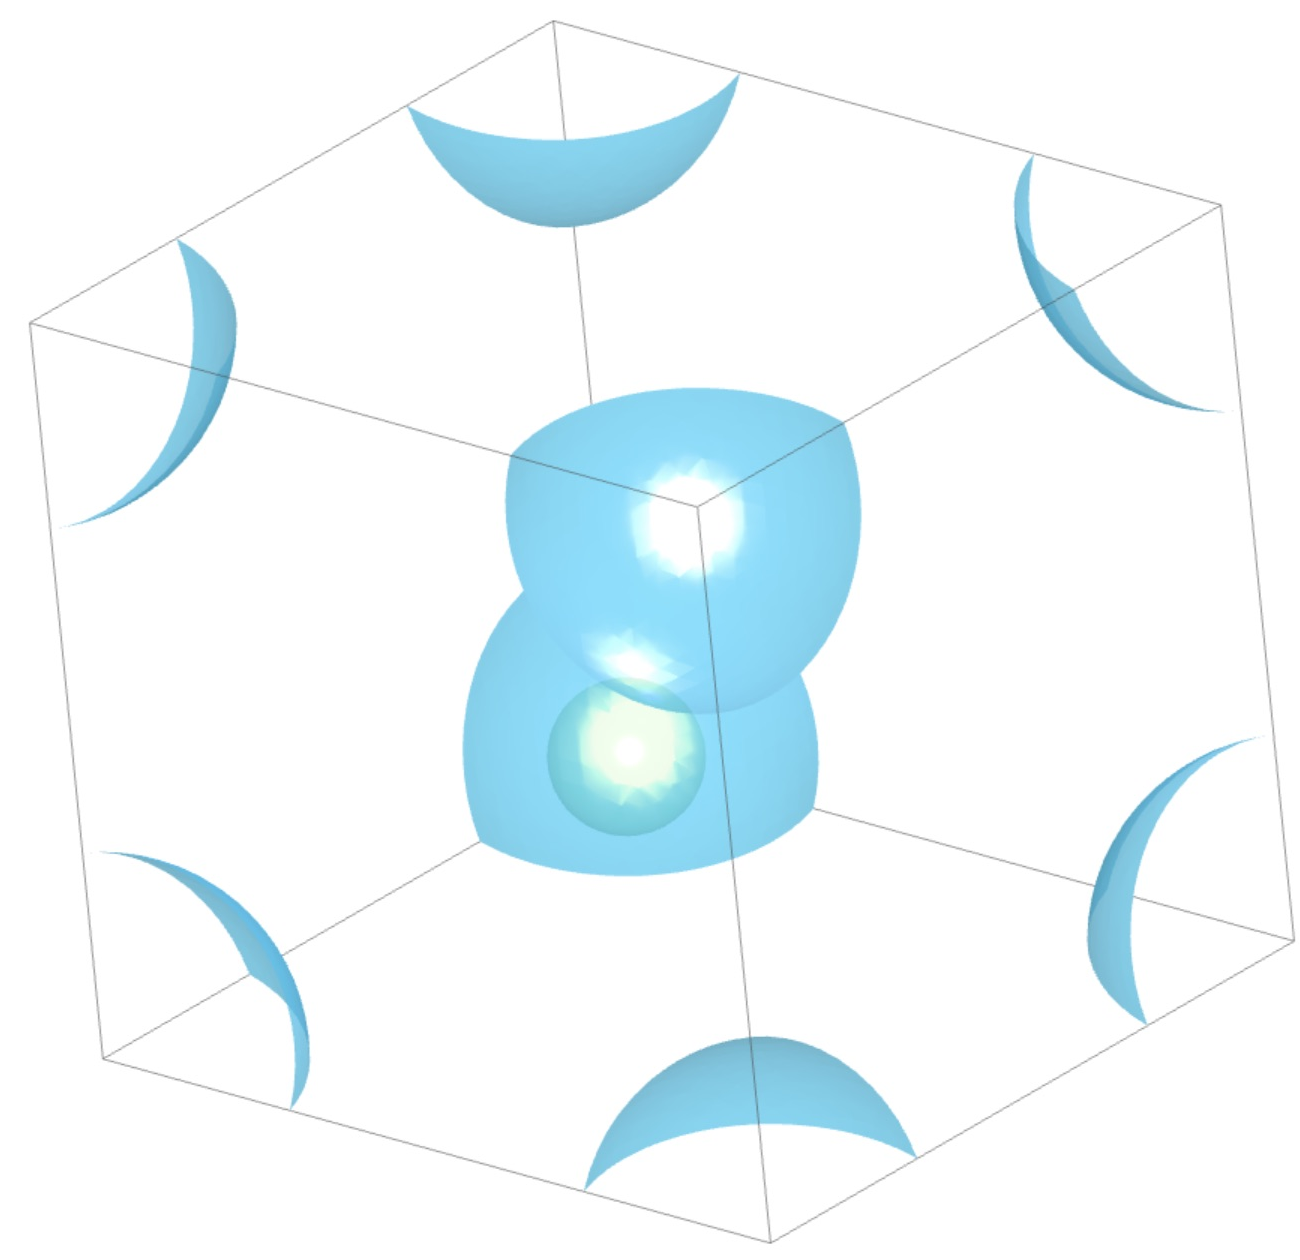
\includegraphics[width=112mm]{publication-assets/crop-53085697480f4dfda16f.png}
\caption{\file{CHGCAR.nospin.gz}的总电荷密度等值面。网格为$32\times32\times32$，通道为\ui{Total charge density}；正阈值为$0.04000\,\text{\AA}^{-3}$，负面关闭，透明度为0.72。}
\label{fig:volume-total-isosurface}
\end{figure}


\section{等值面：观察同一数值形成的形状}
\index{Dengzhimian@等值面}

\subsection{阈值决定看见什么}

等值面连接标量值相同的位置。提高正阈值通常会使显示集中到数值较高的区域，降低阈值则可能使面扩大或相互连通。没有出现等值面时，先查看阈值是否落在数据范围内，以及该通道是否真的具有相应符号。


若以$s(\mathbf r)$表示当前通道的标量场，阈值为$\tau$，对应的等值面就是
\begin{equation}
  S_{\tau}=\{\,\mathbf r\mid s(\mathbf r)=\tau\,\}.
  \label{eq:volume-isosurface}
\end{equation}
它固定的是数值，表面的位置和形状由数据决定。切面则先固定一个空间平面，再用颜色表示平面上各点的$s$值。二者所回答的问题不同，如图\ref{fig:volume-surface-slice-concept}所示；直接体渲染又进一步沿视线组合一段体积中的信息。

\begin{figure}[htbp]
\centering
\begin{tikzpicture}[x=1mm,y=1mm,font=\sffamily\small]
  \node[text=brand] at (25,45) {等值面：固定数值};
  \node[text=brand] at (89,45) {切面：固定位置};
  \foreach \dx in {0,64} {
    \draw[draw=muted!55,line width=.4pt]
      ({5+\dx},4) rectangle ({39+\dx},30);
    \draw[draw=muted!55,line width=.4pt]
      ({5+\dx},30) -- ({14+\dx},38) -- ({48+\dx},38)
      -- ({48+\dx},12) -- ({39+\dx},4);
    \draw[draw=muted!55,line width=.4pt] ({39+\dx},30) -- ({48+\dx},38);
    \draw[dashed,draw=muted!40,line width=.4pt]
      ({5+\dx},4) -- ({14+\dx},12) -- ({48+\dx},12);
    \draw[dashed,draw=muted!40,line width=.4pt]
      ({14+\dx},12) -- ({14+\dx},38);
  }
  \filldraw[fill=teal!25,draw=teal,line width=.7pt]
    (26,21) ellipse (13 and 10);
  \draw[draw=teal!65,dashed,line width=.5pt] (13,21) arc (180:0:13 and 3.2);
  \draw[draw=teal!65,line width=.5pt] (13,21) arc (180:360:13 and 3.2);
  \node[text=brand] at (26,25) {$s=\tau$};
  \filldraw[fill=paleblue,draw=brand,line width=.7pt]
    (69,17) -- (103,8) -- (112,25) -- (78,34) -- cycle;
  \begin{scope}
    \clip (69,17) -- (103,8) -- (112,25) -- (78,34) -- cycle;
    \fill[teal!25] (88,21) ellipse (14 and 11);
    \fill[teal!50] (88,21) ellipse (9 and 7);
    \fill[brand!65] (88,21) ellipse (4 and 3.2);
  \end{scope}
  \draw[draw=brand,line width=.7pt]
    (69,17) -- (103,8) -- (112,25) -- (78,34) -- cycle;
  \node[text=ink] at (25,-4) {形状随场与阈值改变};
  \node[text=ink] at (89,-4) {颜色表示平面上的场值};
\end{tikzpicture}
\caption{同一标量场的两种观察方式（概念示意）。等值面连接相同数值的位置；切面取一个平面，用色彩显示其内部变化。图中几何与色阶仅作概念示意。}
\label{fig:volume-surface-slice-concept}
\end{figure}


在\ui{Display mode} 中选择 \ui{Isosurfaces}。正面与负面分别具有开关和阈值。总电荷密度通常主要观察正面；磁化差、轨道等带符号数据可能需要同时显示两种符号。透明度影响可见程度，不改变阈值和源数据。

\ui{Isovalue units} 提供三种阈值表示方式：绝对数值、标准差和百分位。绝对值适合明确的物理阈值；标准差按均值与分布宽度描述位置；百分位则按数据分布选择阈值。比较两个模型的绝对分布时，应使用相同单位，并明确记录各自阈值。


\ui{Absolute value}按所选显示单位直接填写$\tau$，并不把负值变成正值。选择\ui{Standard deviations (σ)}时，输入的是相对均值的标准差倍数$z$，实际阈值为
\begin{equation}
  \tau=\mu+z\sigma.
  \label{eq:volume-sigma-threshold}
\end{equation}
$\mu$和$\sigma$取自当前通道的网格数值，分别表示均值和标准差。$z=0$对应均值，$z=1$对应均值以上一个标准差，不能直接理解为场值等于1；若通道均值不为零，也不能把阈值简写成$z\sigma$。

\begin{table}[htbp]
\centering
\caption{阈值与颜色范围中的量。}
\begin{tabularx}{\linewidth}{lX}
\toprule
量 & 界面中的意义\\
\midrule
$s$、$\tau$ & 当前通道值和等值面阈值；绝对输入使用通道的显示单位\\
$\mu$、$\sigma$ & 当前通道的均值和标准差；与通道值具有相同单位\\
$z$ & 标准差倍数，无量纲；用于将统计位置换成实际阈值\\
颜色上下限 & 指定色表覆盖的数值区间，不改写场值或CSV数据\\
\bottomrule
\end{tabularx}
\end{table}

\ui{Percentile}按网格样本的数值排序选择阈值。例如第90百分位描述该阈值在样本分布中的位置，并不表示等值面包住了90\%的电子数或晶胞体积。切换通道后，均值、标准差和百分位都会随数据改变，比较两幅图时要同时记录阈值的表示方式。

\subsection{示例：查看总电荷密度}

\begin{steps}
  \item 打开\file{CHGCAR.nospin.gz}，核对摘要中的\ui{Grid}为$32\times32\times32$，\ui{Channel}为\ui{Total charge density}，单位为$\text{\AA}^{-3}$。
  \item 在显示设置中选择\ui{Isosurfaces}，将\ui{Isovalue units}设为\ui{Absolute value}。勾选\ui{Positive}，在其\ui{Threshold}中输入\literalinput{0.04000}。
  \item 关闭\ui{Negative}，将\ui{Opacity}设为\literalinput{0.72}。这样可以透过部分表面辨认内部原子，同时保留等值面的轮廓。
  \item 保留\ui{Atoms}和晶胞，暂时关闭\ui{Bonds}、\ui{Depth Cueing}、\ui{Boundary image atoms}与\ui{One-hop bonded atoms}，使画面集中于场的分布。
  \item 旋转视图，比较晶胞中部与边界附近的等值面。记录文件、通道、单位、阈值与透明度，再导出需要的图像。
\end{steps}

图\ref{fig:volume-total-settings}把摘要与设置分别放大。先用左侧确认读入的数据，再用右侧确认显示条件，便不会把网格大小、密度阈值和透明度混为同一类参数。这里的0.04000适用于本例文件；换用其他数据时，应先查看该通道的数值范围，再选择阈值。

\begin{figure}[H]
\centering
\begin{minipage}[t]{50mm}
\vspace{0pt}
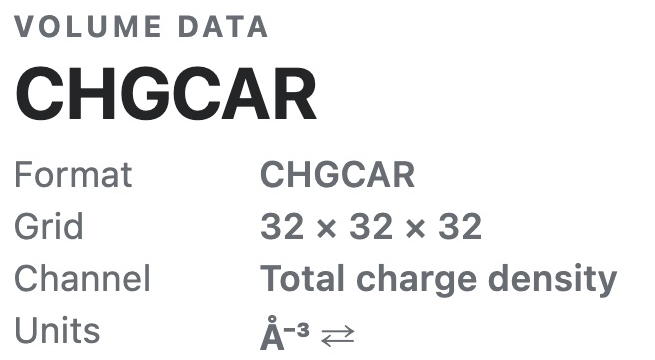
\includegraphics[width=\linewidth]{publication-assets/crop-817224ae41bbaff8bca4.png}
\end{minipage}\hfill
\begin{minipage}[t]{70mm}
\vspace{0pt}
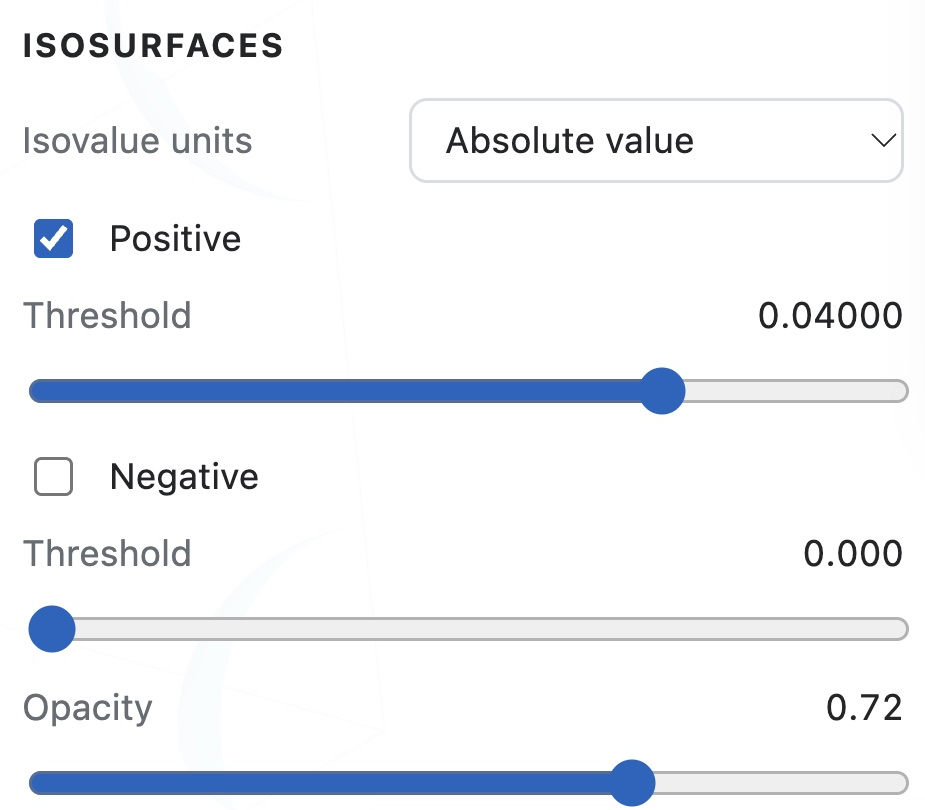
\includegraphics[width=\linewidth]{publication-assets/crop-f580c4c4a5007b46634f.png}
\end{minipage}
\caption{同一总密度视图的摘要与阈值设置。左侧列出网格、通道和单位；右侧采用绝对阈值0.04000，关闭负面，透明度为0.72。}
\label{fig:volume-total-settings}
\end{figure}

\subsection{示例：比较自旋通道}

本例使用\file{CHGCAR.spin.gz}。打开后先查看总密度，再切到\ui{Magnetization density}，即\file{diff}通道。摘要中的网格变为$48\times48\times48$。当前通道在分布图中显示的范围约为$-0.001142$至$-0.0001356\,\text{\AA}^{-3}$，所有数值都在零以下。

\begin{steps}
  \item 在显示设置中选择\ui{Magnetization density}、\ui{Isosurfaces}和\ui{Absolute value}，核对摘要中的通道与单位。
  \item 勾选\ui{Negative}，在它下方的\ui{Threshold}输入\literalinput{-0.0006000}。该值位于本例数据范围内，应出现红色负等值面。
  \item 将\ui{Opacity}设为\literalinput{0.72}，保留原子与晶胞，沿用前例关闭化学键及外围映像的显示设置。转动视图，观察晶胞内部与边界附近的表面。
  \item 可保持\ui{Positive}勾选、阈值为0，如图\ref{fig:volume-diff-settings}。本文件没有零或正值，因此这个开关不会增加正等值面。图中的绿色球体来自原子叠加，与等值面的正负开关分别控制。
  \item 继续切换到\file{up}和\file{down}，查看由总密度与差密度得到的两个自旋通道。每次切换后重新检查数值范围与阈值，并为不同通道分别记录显示条件。
\end{steps}

负磁化密度表示当前自旋约定下的差密度为负，并不表示总电荷密度为负。本例说明负面开关与阈值的关系；若要同时观察正、负两种表面，需要所选数据本身具有相应的取值范围。

\begin{figure}[H]
\centering
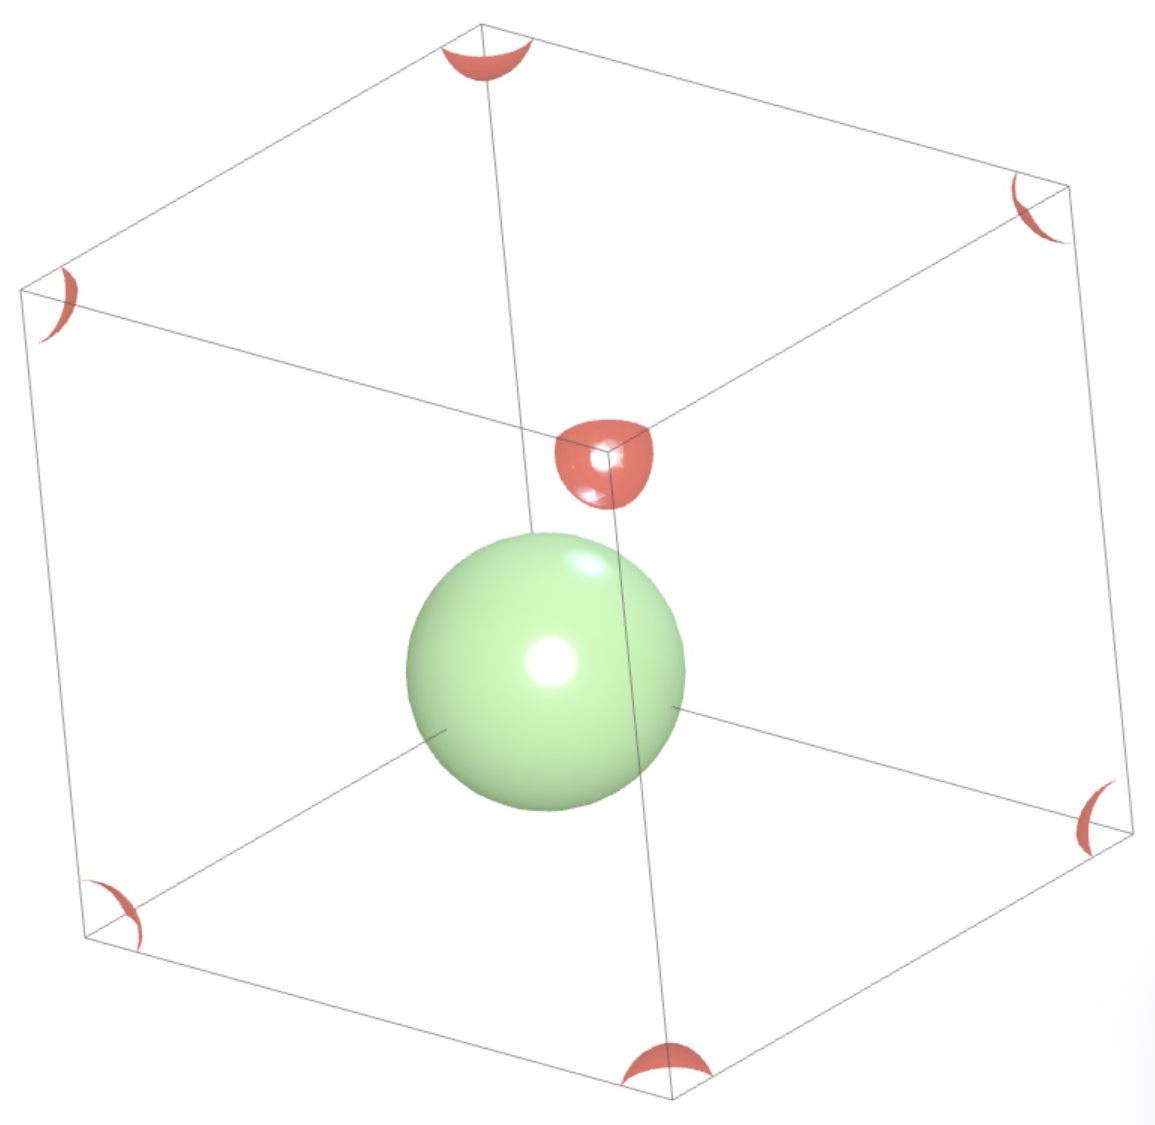
\includegraphics[width=112mm]{publication-assets/crop-eb58a23d11fe997c90a4.png}
\caption{\file{CHGCAR.spin.gz}中\ui{Magnetization density}通道的等值面。网格为$48\times48\times48$，红色表面的阈值为$-0.0006000\,\text{\AA}^{-3}$，透明度为0.72；绿色球体是叠加显示的原子。}
\label{fig:volume-diff-isosurface}
\end{figure}

\begin{figure}[H]
\centering
\begin{minipage}[t]{50mm}
\vspace{0pt}
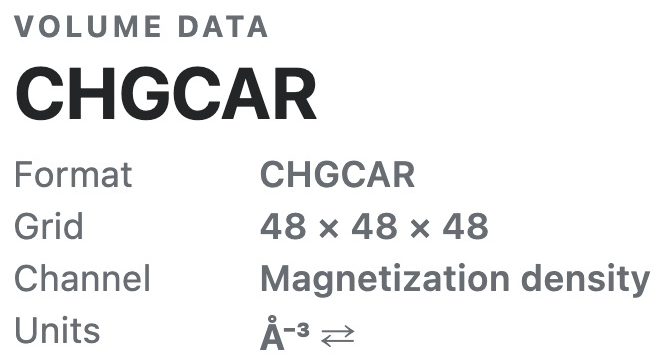
\includegraphics[width=\linewidth]{publication-assets/crop-1252e2f6c064962fc6d9.png}
\end{minipage}\hfill
\begin{minipage}[t]{70mm}
\vspace{0pt}
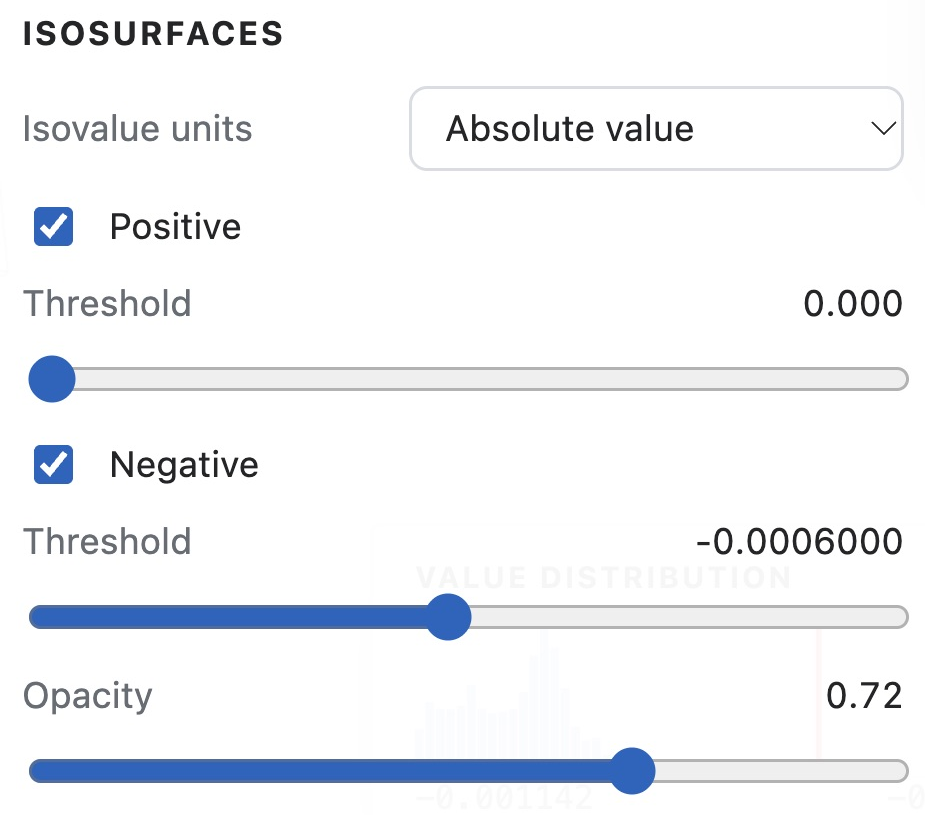
\includegraphics[width=\linewidth]{publication-assets/crop-6e54a4267b5bd8c4b3c0.png}
\end{minipage}
\caption{磁化密度的摘要与阈值设置。正面开关保留在0，负面阈值为$-0.0006000\,\text{\AA}^{-3}$。由于本通道全部为负，只形成负等值面。}
\label{fig:volume-diff-settings}
\end{figure}


\subsection{平滑与周期边界}

\ui{Smooth vertex normals} 改善等值面的光照外观，使三角面片之间的明暗更连续。它不会提高原始网格分辨率。对于周期采样数据，\ui{Wrap periodic boundaries} 可使边界附近的等值面按周期关系连接；是否启用应与文件的周期性一致。

若边界处出现表面截断，先检查晶胞边界和周期设置，再判断是否来自网格本身。使用较高质量的图像导出可以使文字和边缘更清楚，但无法弥补源数据采样过粗的问题。

\section{\headinglatin{Miller} 切面：查看内部数值}
\index{Qiemian@切面}
\index{Miller qiemian@Miller 切面}

\subsection{一个指数组定义一个平面}

等值面适合看形状，切面适合看一个截面内的连续变化。选择 \ui{Miller plane slice} 后，设置中的 I、J、K 共同构成一组 Miller 指数，定义穿过体数据中心的单个平面。三项不能全为 0。

例如 $(0,0,1)$ 与 $(1,0,0)$ 选择不同取向；$(1,1,0)$ 则可观察斜截面。它们是同一个平面的方向参数，不是三张可以独立移动的切片。在非正交网格中，切面按照实际体素矢量确定空间方向，不能把 I、J、K 直接当作笛卡尔 $x$、$y$、$z$ 滑块。


在三个方向均有多个采样点的三维网格中，令$u,v,w$分别表示沿三个网格方向、从首个到末个采样点的归一化位置，范围为0至1。界面中的I、J、K分别记为$h,k,l$，当前中心切面满足
\begin{equation}
  h\left(u-\frac12\right)
  +k\left(v-\frac12\right)
  +l\left(w-\frac12\right)=0.
  \label{eq:volume-central-miller}
\end{equation}
$(0,0,1)$因此给出$w=1/2$；$(1,1,0)$给出$u+v=1$，仍经过网格中心。这里的归一化位置横跨采样范围，不能一概当作完整晶胞的分数坐标。查看器再依据体素矢量把该平面映射到真实空间，所以斜网格也保留相应取向。改变整数组是在改变中心平面的方向，而不是沿某一轴移动它。

\subsection{示例：观察 \headinglatin{Cube} 的(110)切面}

\begin{steps}
  \item 打开\file{elec.cube.gz}，核对摘要中的网格为$23\times23\times24$，通道为\ui{Dataset 1}，单位为\file{arbitrary}。
  \item 在显示设置中选择\ui{Miller plane slice}，将 I、J、K 三个数值分别设为1、1、0。
  \item 在\ui{Colormap}中选择\ui{Cool--warm}，将\ui{Interpolation}设为\ui{Linear}。\ui{Range minimum}保留\literalinput{0.0034185}，把\ui{Range maximum}改为\literalinput{0.2}。
  \item 保留原子与晶胞，将\ui{Atom scale}设为\literalinput{0.22}；关闭化学键、配位多面体、深度明暗及外围映像，使倾斜平面更容易辨认。
  \item 关闭设置面板，转动模型，观察切面穿过晶胞的位置及原子相对于平面的分布。需要比较采样效果时，可切换\ui{Nearest}，观察分块，再恢复\ui{Linear}。
  \item 记录切面指数、色表、颜色范围和插值方式，再从\ui{Slice export}导出PNG或CSV。导出文件的内容见本章后面的导出小节。
\end{steps}

图\ref{fig:volume-miller110}采用较低的颜色上限，使切面中数值较小区域的变化更明显。超过0.2的值使用色表的高端颜色显示，源数据仍保留原值；CSV也不会将它们截为0.2。本例的红蓝表示所选数值区间的两端，不能仅凭颜色判断数值的正负。

\begin{figure}[H]
\centering
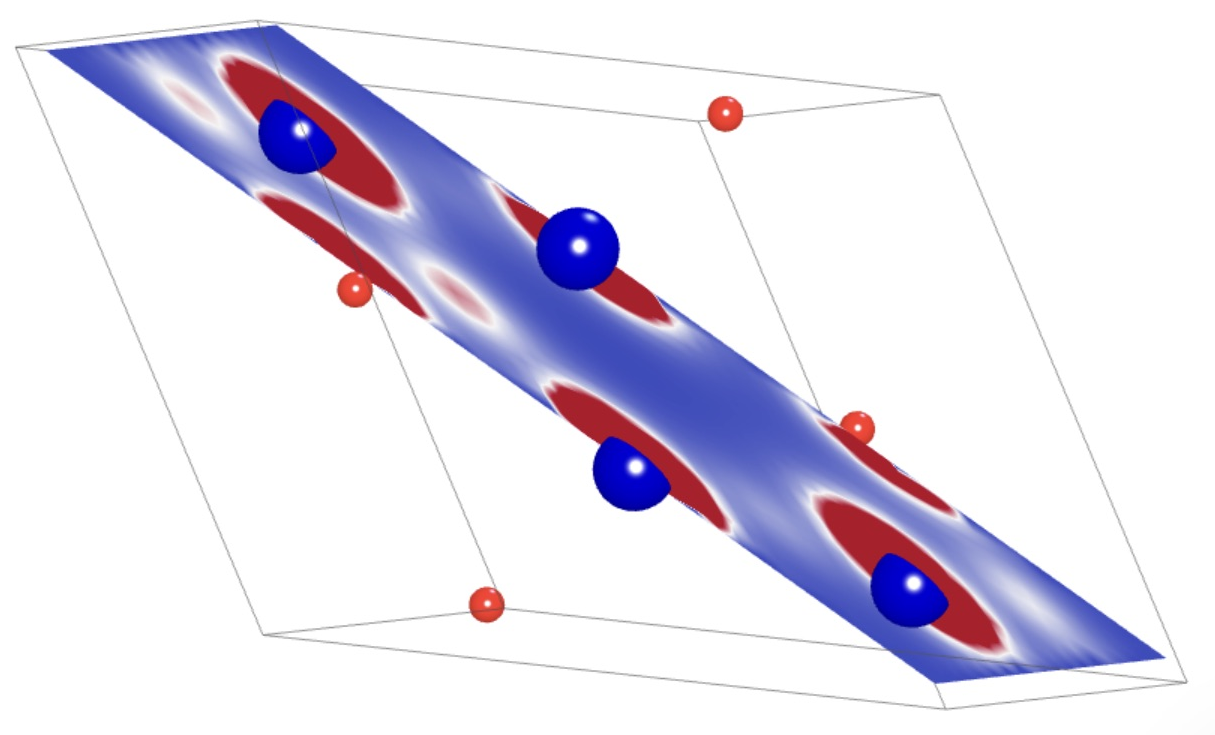
\includegraphics[width=112mm]{publication-assets/crop-aa00ad998951381ace74.png}
\caption{\file{elec.cube.gz}的(110)切面。网格为$23\times23\times24$，通道为\ui{Dataset 1}，标量单位为\file{arbitrary}；采用\ui{Cool--warm}、线性插值和0.0034185至0.2的颜色范围。}
\label{fig:volume-miller110}
\end{figure}

\begin{figure}[H]
\centering
\begin{minipage}[t]{50mm}
\vspace{0pt}
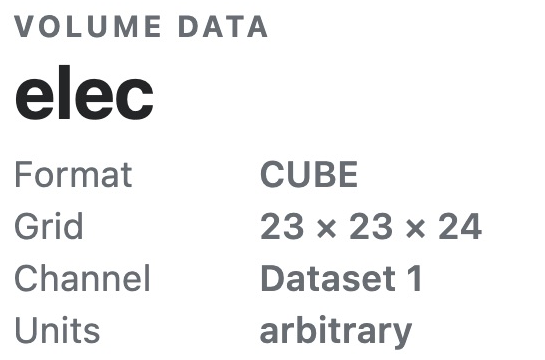
\includegraphics[width=\linewidth]{publication-assets/crop-ab9df592529bd047787b.png}
\end{minipage}\hfill
\begin{minipage}[t]{70mm}
\vspace{0pt}
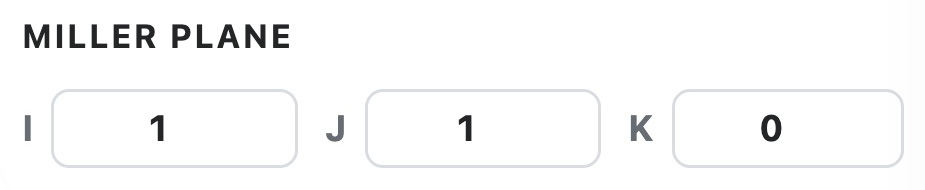
\includegraphics[width=\linewidth]{publication-assets/crop-1de9d3c6e62d7816cea2.png}
\par\vspace{2mm}
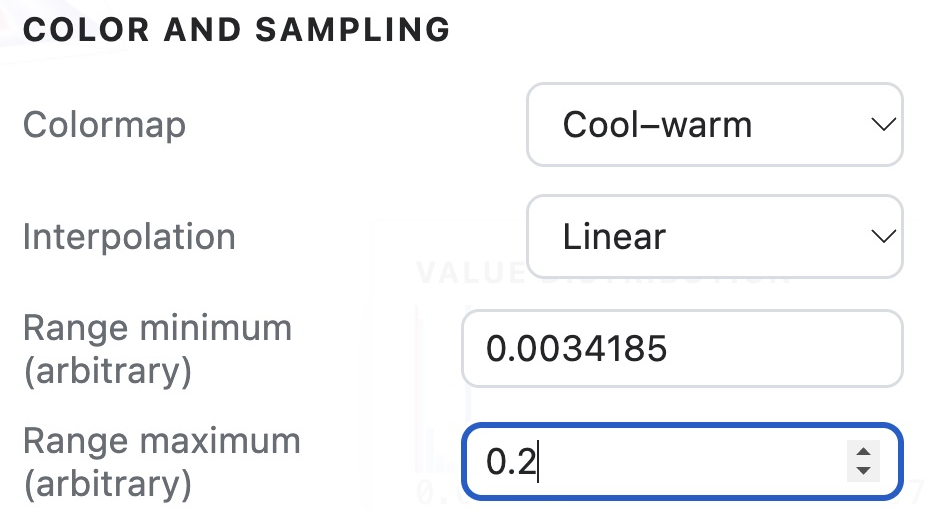
\includegraphics[width=\linewidth]{publication-assets/crop-209a06fc6024f4d5e0ba.png}
\end{minipage}
\caption{切面摘要和设置局部。左侧核对文件、网格与单位；右侧上方填写同一组Miller指数，下方设置色表、插值及颜色范围。颜色上限0.2只控制显示。}
\label{fig:volume-miller110-settings}
\end{figure}

还可以打开\file{datagrid_3d.xsf}，先按标签辨认通道，再重复切面练习。比较两个文件时，既看网格的空间取向，也看标量本身的含义；相同的(110)指数并不要求两张图具有相同尺寸或数值范围。


\subsection{颜色范围与分布图}

\ui{Range minimum} 和 \ui{Range maximum} 决定哪些数值映射到色表两端。范围较宽时，局部变化可能不明显；适当缩小范围可以突出感兴趣的区间。超出颜色范围的值仍然存在，只是采用端点颜色显示。

\ui{Value Distribution} 展示当前通道的数值分布。在等值面模式中，点击分布图可以设置相应正、负阈值；在切面或直接体渲染中，点击则调整较近的颜色范围端点，也可拖动标记细调。它是选择显示区间的工具，不是能谱，也不是沿某条空间路径的剖面。

对于带正负的场，\ui{Cool--warm} 常便于辨认两侧；对于非负场，连续色表通常更容易阅读。比较不同模型时应尽量保持同一色表与颜色范围，使颜色差异具有相同含义。

\section{直接体渲染与结构叠加}
\index{Zhijie ti xuanran@直接体渲染}

直接体渲染沿视线累积标量场的颜色与透明度，可以同时看到较大范围的内部变化。在\ui{Display mode} 中选择 \ui{Direct volume (GPU)}，再按需要调整透明度、梯度透明度和采样质量。\ui{Fast} 适合交互观察，\ui{Balanced} 用于一般查看，\ui{High} 适合在设备允许时检查细节。

I、J、K 的裁剪上下限以 0 到 1 的比例表示，可去掉盒子的一部分，使内部更易观察。例如，将一个方向的范围从 0--1 缩到 0.25--0.75，可以聚焦中部区域。裁剪改变显示范围，不会删除文件中的数据。

\subsection{示例：沿网格方向查看中部体积}

继续使用前例的\file{elec.cube.gz}，便于比较同一份数据在切面和体渲染中的不同表现。切面显示一个平面上的数值，体渲染则沿视线叠加一段体积中的颜色与透明度，因此两种模式的明暗不必逐点相同。

\begin{steps}
  \item 核对文件仍为\file{elec.cube.gz}，通道为\ui{Dataset 1}，网格为$23\times23\times24$，单位为\file{arbitrary}。将\ui{Display mode}切换为\ui{Direct volume (GPU)}。
  \item 沿用\ui{Cool--warm}、\ui{Linear}及0.0034185至0.2的颜色范围。先保持颜色设置一致，再比较显示方式。
  \item 将\ui{Sampling quality}设为\ui{Balanced}，\ui{Opacity}设为\literalinput{0.72}，\ui{Gradient opacity}设为\literalinput{0.35}。后者调整局部变化对透明度的影响，可与整体透明度分别试调。
  \item 将\ui{I clipping}的下限与上限分别设为\literalinput{0.25}、\literalinput{0.75}；\ui{J clipping}与\ui{K clipping}均保留0和1。此时只显示I方向中间一半的体积，另外两个网格方向保持完整。
  \item 保留原子与晶胞，关闭化学键、多面体及外围映像。关闭设置面板并按I隐藏摘要与分布图，转动视图观察内部的连续变化。需要核对文件信息时，再按I恢复辅助界面。
\end{steps}

图\ref{fig:volume-direct}展示直接体渲染效果，设置局部见图\ref{fig:volume-direct-settings}。I、J、K在这里表示网格方向上的裁剪比例，与前节Miller切面的整数组定义不同；它们也不一定与全局笛卡尔坐标轴重合。将裁剪恢复为0至1即可重新显示完整体积，源网格仍为$23\times23\times24$。

\begin{figure}[H]
\centering
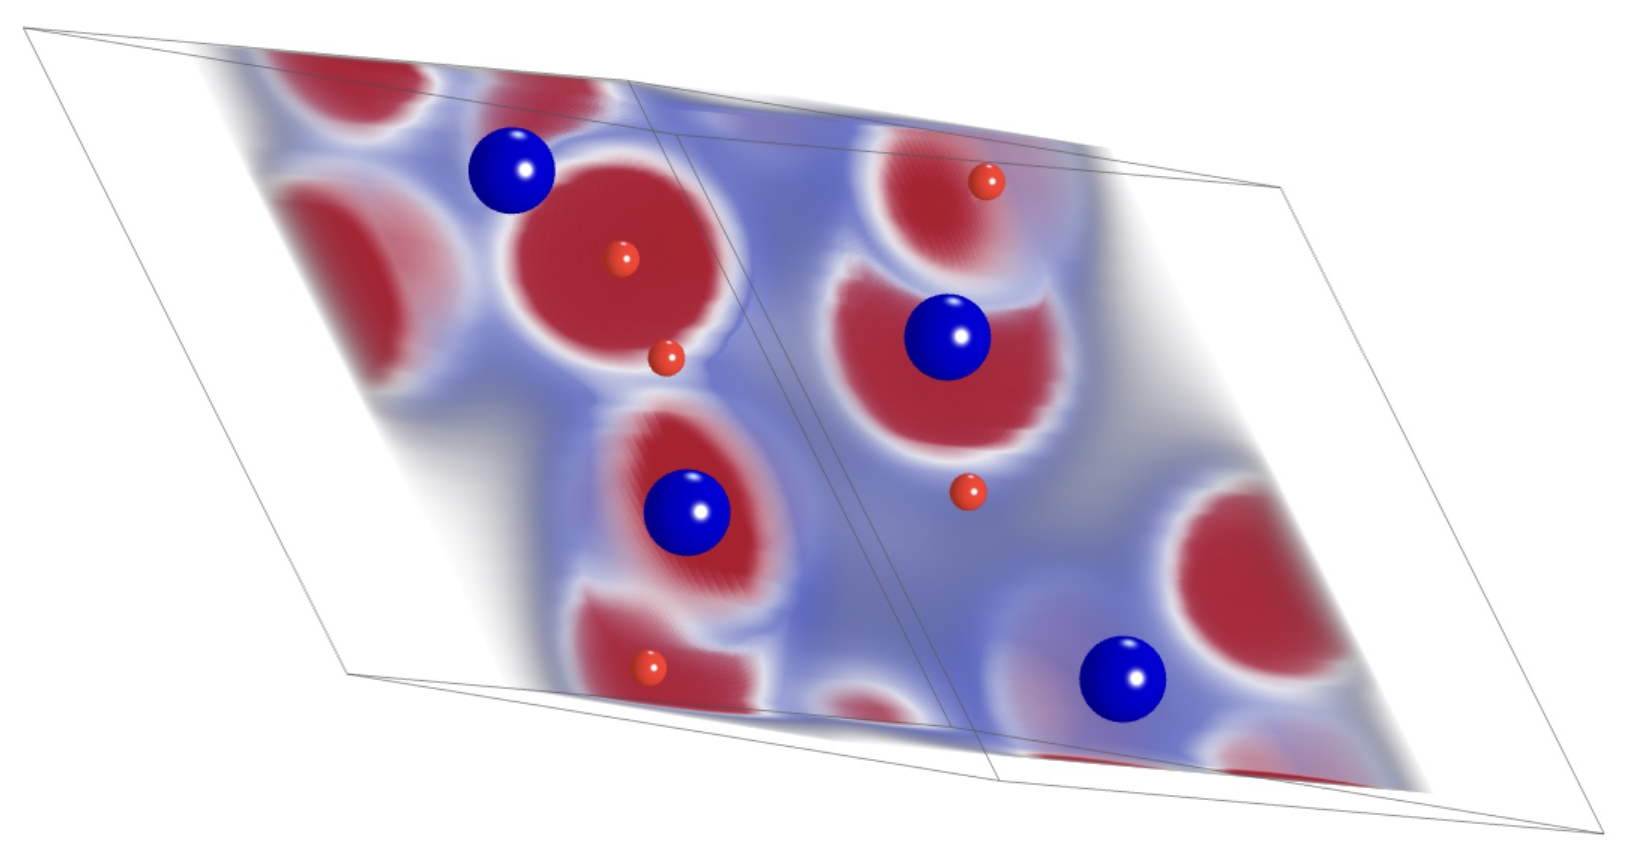
\includegraphics[width=112mm]{publication-assets/crop-68bb0517e51ea1057170.png}
\caption{\file{elec.cube.gz}的直接体渲染画面。显示模式为\ui{Direct volume (GPU)}；\ui{Dataset 1}的颜色范围为0.0034185至0.2，I方向显示0.25至0.75，原子与完整晶胞轮廓用于定位。}
\label{fig:volume-direct}
\end{figure}

\begin{figure}[H]
\centering
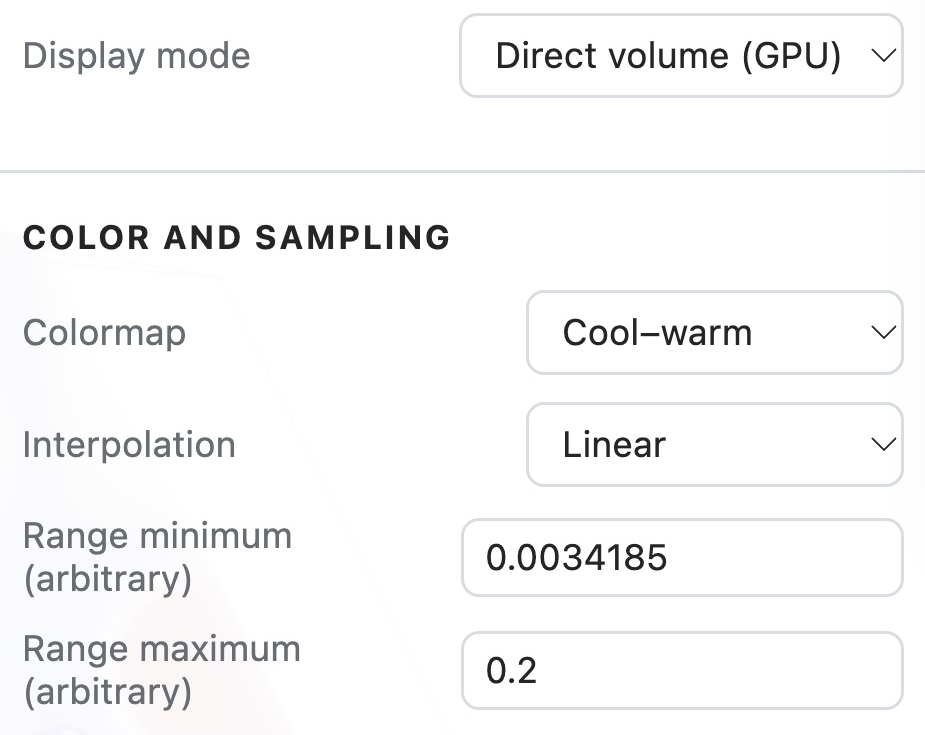
\includegraphics[width=80mm]{publication-assets/crop-3b2d9027085c84d05818.png}
\par\vspace{2mm}
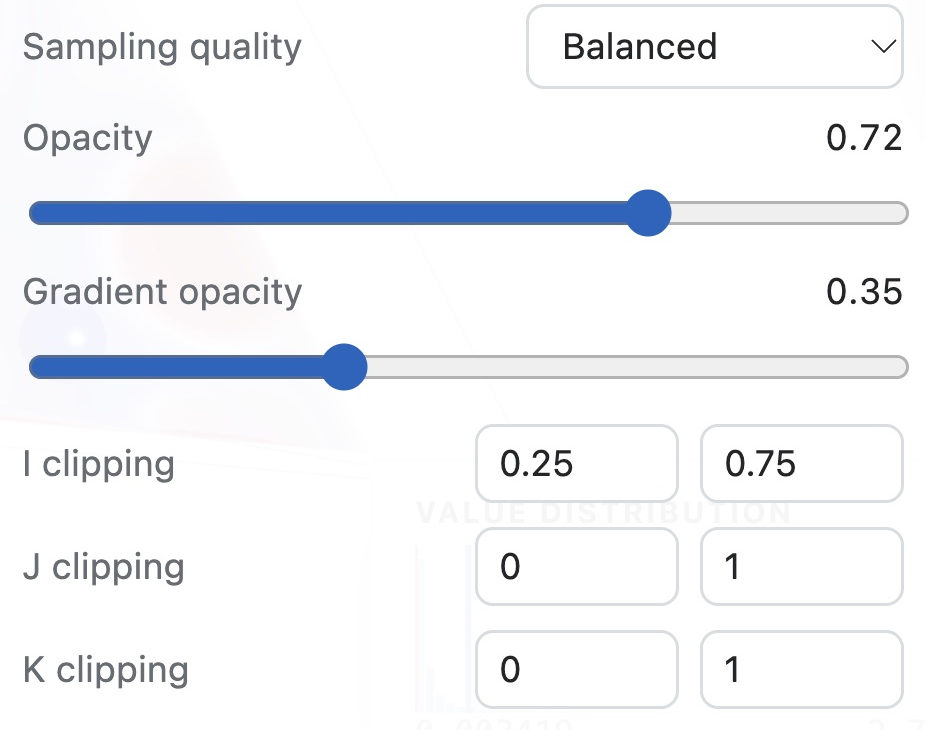
\includegraphics[width=80mm]{publication-assets/crop-7567d94dfd7d877833b9.png}
\caption{直接体渲染设置。上方为模式、色表、插值和颜色范围；下方为\ui{Balanced}采样质量、0.72透明度、0.35梯度透明度及三个方向的裁剪比例。}
\label{fig:volume-direct-settings}
\end{figure}

\subsection{用结构叠加定位场}

若体数据包含原子结构，\ui{Visibility} 中可以控制原子、化学键、晶胞、配位多面体、方向轴、周期边界原子及磁矩等对象。先保留用于定位的少量对象，再逐一增加辅助显示，通常更容易看清场与结构的关系。

\ui{Lighting \& surface} 控制原子叠加的环境光、方向光、金属度、粗糙度、亮度和对比度。它们影响图像外观，不改变标量场的大小。制作一组比较图时，保持这些设置一致，并把决定科学含义的通道、阈值和单位写入图注。


\section{导出体数据}
\index{Daochu tuxiang yu shuju@导出图像与数据}

\subsection{在视图中采样}
\index{Caiyang@采样数值}

双击体数据可以显示采样值与网格位置。点探针使用三线性插值，数值不一定等于某一个原始网格点。需要精确比较时，应记录通道与采样位置，并使用采样数值。切面中的最近邻或线性选项另用于切面显示与导出，不改变点探针的插值方式。

选择叠加原子时，体数据视图内的原子信息区域可显示笛卡尔与分数坐标，复制按钮保留比面板简写更多的数值精度。原子坐标与标量采样是不同的信息：一个用于定位原子，一个用于读取空间场。

对于可转换的密度单位，\ui{Density units} 可在 $\text{\AA}^{-3}$ 与 $\mathrm{bohr}^{-3}$ 之间切换。切换单位会改变显示数值，所代表的物理密度保持相同。比较图表和报告时，统一单位后再比较数值。

\subsection{导出当前图像}

图像导出菜单提供 PNG、JPEG、TIFF、SVG，以及向量和栅格两类 PDF。PNG 和 TIFF 适合保留清晰的栅格图；JPEG 便于压缩分享；SVG 和 PDF 适合插入排版流程。导出前先停止自动旋转，选定取景，确认希望保留的原子、晶胞和辅助对象。

导出图像时，在正文或图注写明文件来源、通道、阈值或颜色范围、单位与必要取向，并保留相应原始数据。

\subsection{导出等值面和切面}
\index{CSV@CSV 导出}

在等值面模式下，\ui{Isosurface export} 提供 glTF、GLB、PLY 和 STL，用于把当前等值面几何送入其他三维工具。不同格式保存的信息不完全相同；使用外部软件后应核对尺寸和外观，坐标按 \AA 理解。

在切面模式下，\ui{Slice export} 提供 PNG 和 CSV。切面 PNG 用于保存当前平面的颜色图；CSV 用于后续作图或数值分析。CSV 先列出网格位置 \file{i}、\file{j}、\file{k}，再列出以 \AA 为单位的笛卡尔位置 \mbox{\file{x_angstrom}}、\mbox{\file{y_angstrom}}、\mbox{\file{z_angstrom}}，最后是当前通道的源数值 \file{value}。切面边界外的采样位置可能没有有效值，分析时应按数据有效范围处理。

导出后可以做一次简单核对：重新打开 PNG，确认取向、色表和感兴趣区域；再查看 CSV 表头，确认坐标单位与数值列。若希望把两套模型的同一切面画在同一张图中，应先保证切面的空间定义、网格范围和通道一致。相同的 Miller 指数给出相同类型的方向，但晶胞改变后，平面的真实尺寸和经过的位置仍可能不同。

本例导出文件为\file{elec.total.slice-1_1_0.csv}与同名PNG。CSV有1568个采样位置，其中778个具有有限数值，另790个在体数据边界外，\file{value}记为\file{NaN}。NaN不表示数值为零，作图或统计时应先筛选有效值。

这些有效切面值约为0.003525至2.3995，其中147个仍大于显示上限0.2，可以用来核对颜色设置与源数值的区别。切面PNG为$384\times768$像素，显示采样平面中的颜色分布；图\ref{fig:volume-miller110}同时呈现切面在晶胞中的取向。

\Needspace{8\baselineskip}
\begin{notebox}{显示单位与 CSV}
CSV 的坐标列以 \AA 输出，数值列保留通道内部采用的单位。对于 \mbox{CHGCAR}，密度数值按 $\text{\AA}^{-3}$ 理解；界面切换为 $\mathrm{bohr}^{-3}$ 时，CSV 数值列仍使用 $\text{\AA}^{-3}$。Cube 和 XSF 的标量单位则应按源文件说明记录。
\end{notebox}

\ui{Export scene JSON} 导出场景描述，便于保留网格、通道及结构等说明信息。它不包含完整体素数组，也不能代替保存原始场文件；相机位置和临时显示设置需另行记录。需要重现图像时，另记阈值、颜色范围和取景，并同时保留原始数据。

\subsection{组织一组可比较的结果}

完成一次观察后，可以为数据与图像建立对应名称，例如在文件名中包含体系、通道和切面。对 CHGCAR 的 \file{total} 与 \file{diff} 分别保留图像，避免用“密度图”概括含义不同的通道。在图注中说明正负面的颜色和阈值；在切面图中说明颜色范围。读者无需打开原文件，也应能判断图上颜色和表面代表什么。

若图形用于研究报告，可保留一张带完整摘要和设置的工作截图，再导出一张布局整洁的结果图。前者便于自己复查，后者用于正文展示。最终选择应围绕要说明的现象：等值面强调形状和连接，切面强调局部变化，体渲染强调空间层次，三者各有用处。

\section{图像没有按预期出现时}

等值面为空，先检查通道、正负面开关和阈值范围。切面颜色几乎一致，查看颜色范围是否过宽。原子遮挡场，减小原子比例或暂时隐藏化学键和多面体。旋转后找不到模型，按空格键重新居中。

直接体渲染需要相应的图形支持。若设备不能使用 WebGL2，查看器可采用 CPU 切片方式，并继续提供切片 PNG/CSV 导出；三维纹理容量不足时也可能回到切面。界面显示的降级原因有助于选择当前设备可用的模式。二维XSF使用切面显示。

最后，插值、平滑和更大的导出图片都只改善显示。若研究问题需要更细的空间信息，应回到计算阶段提高源网格分辨率，再重新检查收敛。这样，图像中的细节才有相应数据作为依据。
